\documentclass[tikz,border=10pt]{standalone}
\begin{document}

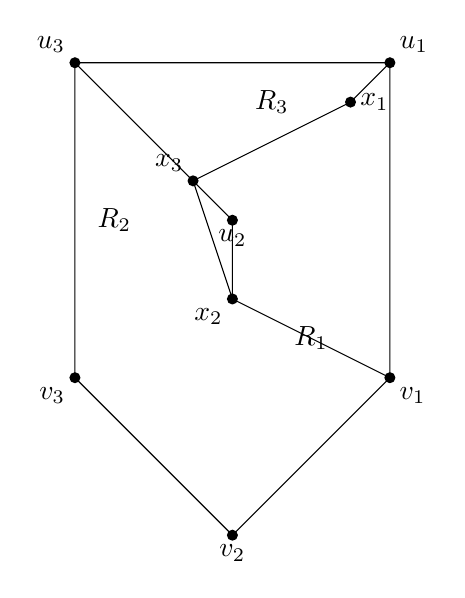
\begin{tikzpicture}
    % Define coordinates
    \coordinate (u1) at (2, 2);
    \coordinate (u2) at (0, 0);
    \coordinate (u3) at (-2, 2);
    \coordinate (v1) at (2, -2);
    \coordinate (v2) at (0, -4);
    \coordinate (v3) at (-2, -2);
    
    \coordinate (x1) at (1.5, 1.5);
    \coordinate (x2) at (0, -1);
    \coordinate (x3) at (-0.5, 0.5);
    
    % Draw hexagon edges
    \draw (u1) -- (v1) -- (v2) -- (v3) -- (u3) -- (u1);
    
    % Draw internal lines
    \draw (u1) -- (x1) -- (x3) -- (u2) -- (x2) -- (x3);
    \draw (u3) -- (x3);
    \draw (x2) -- (v1);
    
    % Draw the dots
    \foreach \i in {u1,u2,u3,v1,v2,v3,x1,x2,x3} {
        \fill (\i) circle (2pt);
    }
    
    % Label vertices
    \node[above right] at (u1) {$u_1$};
    \node[below] at (u2) {$u_2$};
    \node[above left] at (u3) {$u_3$};
    \node[below right] at (v1) {$v_1$};
    \node[below] at (v2) {$v_2$};
    \node[below left] at (v3) {$v_3$};
    
    % Label x-coordinates
    \node[right] at (x1) {$x_1$};
    \node[below left] at (x2) {$x_2$};
    \node[above left] at (x3) {$x_3$};
    
    % Label regions
    \node at (0.5, 1.5) {$R_3$};
    \node at (1, -1.5) {$R_1$};
    \node at (-1.5, 0) {$R_2$};
\end{tikzpicture}

\end{document}